\section{The immersed boundary method}\label{sec:ib}

\subsection{Overview}
\label{sec:ib_old}
Consider a rectangular domain, $\domain\subset\R^3$, which contains one or more
deformable structures and is otherwise filled with an incompressible, Newtonian fluid
with constant density, $\density$, and viscosity, $\viscosity$. The IB method treats
these structures as an extension of the fluid. The motion of any particle in $\domain$ is
therefore governed by the incompressible Navier-Stokes equations,
\begin{gather}
    \density(\u_t + \div(\u\otimes\u)) = \viscosity\laplacian \u - \grad p + \f, \label{eq:ins-momentum} \\
    \div \u = 0, \label{eq:ins-incomp}
\end{gather}
where, for $\x = (x,\,y,\,z) \in \domain$, $\u = \u(\x,\,t) = (u, v, w)$ is the fluid
velocity, $p = p(\x,\,t)$ is the pressure, and $\f = \f(\x,\,t)$ is an external force
density. Here and throughout this paper, we use bold italic symbols to indicate a vector
in $\R^3$. Treating the entire domain as a fluid allows us to discretize $\domain$
independently of the immersed structures with a fixed regular grid of spacing $h$. This
is the Eulerian grid.


Let $\X = \X(\theta,\,\varphi,\,t)$, for surface coordinates $(\theta,\,\varphi)$ in
$\sites\subset\mathbb{R}^2$, be a parametrization for the immersed boundary $\interface$.
Though the interface changes with time, we suppress the time argument $t$ for brevity. A
discrete representation of the boundary, consisting of a set of surface points, replaces
its continuous counterpart.  Surface points are typically chosen to be within
approximately $h$ of their neighbors.  This is the Lagrangian grid. These boundary points
move at the local fluid velocity.  Analytically convolving the fluid velocity against the
Dirac delta function, $\Dirac(\x)$, yields the velocity of a surface point, but
discretely, Eulerian and Lagrangian grid points are unlikely to coincide. The IB method
replaces the singular Dirac delta function with a smoothed, $h$-dependent analogue,
$\Dirac_h(\x)$. The Lagrangian point $\X$ evolves according to
\begin{equation}\label{eq:ib-interp}
    \vec{\dot{X}}
        = \int\limits_{\domain} \u(\x) \Dirac(\x-\X) \d\x
        \approx h^3 \sum_{i} \u(\x_i) \Dirac_h(\x_i-\X),
\end{equation}
where $i$ enumerates the Eulerian grid points, and a superposed dot denotes partial
differentiation with respect to $t$. As a boundary deforms, it generates a force density
$\F = \F(\X,\,t)$, which it imparts onto the fluid as $\f$ in~\eqref{eq:ins-momentum}.
Again, we suppress $t$ when using $\F$. By similar reasoning as the velocity, $\F$ is
transferred to the fluid at $\x$ via
\begin{equation}\label{eq:ib-spread}
        \f(\x)
        = \int\limits_{\interface} \F(\X)\Dirac(\x-\X) \d\X
        \approx \sum_{j} \weight[j]\F(\X_j) \Dirac_h(\x-\X_j),
\end{equation}
where $j$ enumerates the Lagrangian grid points, and $\weight[j]$ is the integration
weight corresponding to Lagrangian grid point $\X_j$. 

In addition to a velocity vector field, equation~\eqref{eq:ib-spread} illustrates the
need for three pieces of information for each immersed structure: the position of points
$\X_j$ used to evaluate forces on the structure; a force density $\F(\X_j)$ at each of
those points; and surface integration weights $\weight[j]$ for those points. Equation~%
\eqref{eq:ib-interp} tells us how to move the structure. The next three sections describe
our methods for solving~\eqref{eq:ins-momentum}--\eqref{eq:ins-incomp} (Section 3), give analytic
expressions for energy functionals used to derive $\F$ (Section 4 and Appendix b), and detail the discretization of the structures to obtain $\X_j$,
$\F(\X_j)$, and $\weight[j]$ (Section 5). However, before we do so, we discuss the specific variant
of the IB method employed herein.

\subsection{The RBF-IB method}
\label{sec:rbfib}
The classical IB method uses the same the Lagrangian points in Equations~\eqref{eq:ib-interp} and~\eqref{eq:ib-spread}. However, there exist several IB methods
use different sets of points instead. For instance, the method in~\cite{Griffith:2017id} uses a finite element representation for the structure, and consequently spreads forces from (Lagrangian)
quadrature points, interpolates velocities to quadrature points, and then projects them using the finite element basis to the nodes. The RBF-IB method used in this work also does something similar. A small set of $\data\cardinality$ Lagrangian points approximately $2h$ apart is used to approximate $\X$ and this set of points is moved by~\eqref{eq:ib-interp}. In addition, a larger set of $\sample\cardinality$ points chosen to be approximately $h$ apart is used to spread forces using~\eqref{eq:ib-spread}. While the former set is widely spaced, the spacing of the latter set of points aligns with traditional IB implementations.

This potentially raises certain concerns, which we address here. The first major concern relates to the force-spreading and velocity interpolation operations. In traditional IB methods, these operators are formally adjoint, leading to conservation of energy/power~\cite{peskin:2002}. However, in the RBF-IB method, these operators are no longer adjoint, leading to concerns about numerical stability. In previous work~\cite{Shankar2015:km}, the authors demonstrated that the RBF-IB method dissipated energy in 2D simulations as expected, despite the absence of formal adjointness. In this work, we show similar results for an RBC relaxation problem in a full 3D simulation. The second major concern related to the wide $2h$ spacing of the smaller set of points used to approximate $\X$ and update the structure. 



\section{Solution of the incompressible Navier-Stokes equations}\label{sec:ins}

\begin{figure}[htb]
    \centering
    \begin{subfigure}{0.33\textwidth}
        \centering
    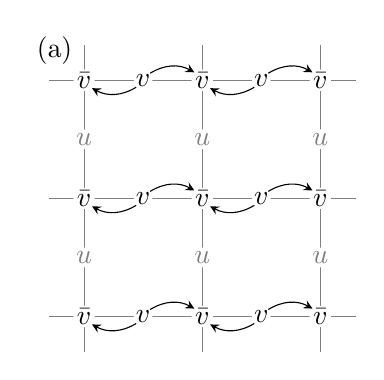
\begin{tikzpicture}[scale=1.5]
        \draw[help lines] (-0.3, -0.3) grid (2.3, 2.3);

        \foreach \x in {0,...,2}
            \foreach \y in {0,...,1}
            {
                \node[circle, inner sep=0pt, color=black!50, fill=white] at (\x, \y+0.5) {$u$};
            }
        \foreach \y in {0,...,2}
        {
            \foreach \x in {0,...,2}
                \node[circle, inner sep=0pt, fill=white] (av\x\y) at (\x, \y) {$\bar{v}$};
            \foreach \x in {0,...,1}
                \node[circle, inner sep=0pt, fill=white] (v\x\y) at (\x+0.5, \y) {$v$};
        }
        \path[-stealth] (v00.south west) edge[bend left] node[midway, below, yshift=+1pt] {} (av00.south east);
        \path[-stealth] (v10.south west) edge[bend left] node[midway, below, yshift=+1pt] {} (av10.south east);
        %\path[-stealth] (v20.south west) edge[bend left] node[midway, below, yshift=+1pt] {} (av20.south east);
        \path[-stealth] (v01.south west) edge[bend left] node[midway, below, yshift=+1pt] {} (av01.south east);
        \path[-stealth] (v11.south west) edge[bend left] node[midway, below, yshift=+1pt] {} (av11.south east);
        %\path[-stealth] (v21.south west) edge[bend left] node[midway, below, yshift=+1pt] {} (av21.south east);
        \path[-stealth] (v02.south west) edge[bend left] node[midway, below, yshift=+1pt] {} (av02.south east);
        \path[-stealth] (v12.south west) edge[bend left] node[midway, below, yshift=+1pt] {} (av12.south east);
        %\path[-stealth] (v22.south west) edge[bend left] node[midway, below, yshift=+1pt] {} (av22.south east);
        %\path[-stealth] (v03.south west) edge[bend left] node[midway, below, yshift=+1pt] {} (av03.south east);
        %\path[-stealth] (v13.south west) edge[bend left] node[midway, below, yshift=+1pt] {} (av13.south east);
        %\path[-stealth] (v23.south west) edge[bend left] node[midway, below, yshift=+1pt] {} (av23.south east);

        \path[-stealth] (v00.north east) edge[bend left] node[midway, below, yshift=+1pt] {} (av10.north west);
        \path[-stealth] (v10.north east) edge[bend left] node[midway, below, yshift=+1pt] {} (av20.north west);
        %\path[-stealth] (v20.north east) edge[bend left] node[midway, below, yshift=+1pt] {} (av30.north west);
        \path[-stealth] (v01.north east) edge[bend left] node[midway, below, yshift=+1pt] {} (av11.north west);
        \path[-stealth] (v11.north east) edge[bend left] node[midway, below, yshift=+1pt] {} (av21.north west);
        %\path[-stealth] (v21.north east) edge[bend left] node[midway, below, yshift=+1pt] {} (av31.north west);
        \path[-stealth] (v02.north east) edge[bend left] node[midway, below, yshift=+1pt] {} (av12.north west);
        \path[-stealth] (v12.north east) edge[bend left] node[midway, below, yshift=+1pt] {} (av22.north west);
        %\path[-stealth] (v22.north east) edge[bend left] node[midway, below, yshift=+1pt] {} (av32.north west);
        %\path[-stealth] (v03.north east) edge[bend left] node[midway, below, yshift=+1pt] {} (av13.north west);
        %\path[-stealth] (v13.north east) edge[bend left] node[midway, below, yshift=+1pt] {} (av23.north west);
        %\path[-stealth] (v23.north east) edge[bend left] node[midway, below, yshift=+1pt] {} (av33.north west);

        \node[black] at (-0.25, 2.25) {(a)};
    \end{tikzpicture}
    \label{fig:adv-x-ave}
    \end{subfigure}%
    \begin{subfigure}{0.33\textwidth}
        \centering
    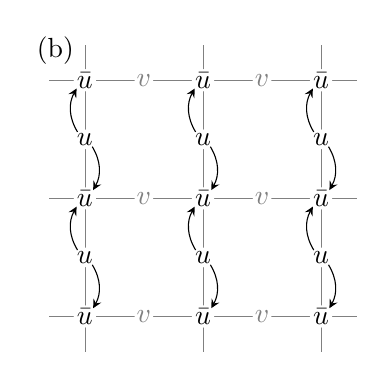
\begin{tikzpicture}[scale=1.5]
        \draw[help lines] (-0.3, -0.3) grid (2.3, 2.3);

        \foreach \x in {0,...,2}
        {
            \foreach \y in {0,...,1}
            {
                \node[circle, inner sep=0pt, fill=white] (u\x\y) at (\x, \y+0.5) {$u$};
            }
            \foreach \y in {0,...,2}
            {
                \node[circle, inner sep=0pt, fill=white] (au\x\y) at (\x, \y) {$\bar{u}$};
            }
        }
        \foreach \x in {0,...,1}
            \foreach \y in {0,...,2}
            {
                \node[circle, inner sep=0pt, color=black!50, fill=white] at (\x+0.5, \y) {$v$};
            }

        \path[-stealth] (u00.south east) edge[bend left] node[midway, below, yshift=+1pt] {} (au00.north east);
        \path[-stealth] (u10.south east) edge[bend left] node[midway, below, yshift=+1pt] {} (au10.north east);
        \path[-stealth] (u20.south east) edge[bend left] node[midway, below, yshift=+1pt] {} (au20.north east);
        %\path[-stealth] (u30.south east) edge[bend left] node[midway, below, yshift=+1pt] {} (au30.north east);
        \path[-stealth] (u01.south east) edge[bend left] node[midway, below, yshift=+1pt] {} (au01.north east);
        \path[-stealth] (u11.south east) edge[bend left] node[midway, below, yshift=+1pt] {} (au11.north east);
        \path[-stealth] (u21.south east) edge[bend left] node[midway, below, yshift=+1pt] {} (au21.north east);
        %\path[-stealth] (u31.south east) edge[bend left] node[midway, below, yshift=+1pt] {} (au31.north east);
        %\path[-stealth] (u02.south east) edge[bend left] node[midway, below, yshift=+1pt] {} (au02.north east);
        %\path[-stealth] (u12.south east) edge[bend left] node[midway, below, yshift=+1pt] {} (au12.north east);
        %\path[-stealth] (u22.south east) edge[bend left] node[midway, below, yshift=+1pt] {} (au22.north east);
        %\path[-stealth] (u32.south east) edge[bend left] node[midway, below, yshift=+1pt] {} (au32.north east);

        \path[-stealth] (u00.north west) edge[bend left] node[midway, below, yshift=+1pt] {} (au01.south west);
        \path[-stealth] (u10.north west) edge[bend left] node[midway, below, yshift=+1pt] {} (au11.south west);
        \path[-stealth] (u20.north west) edge[bend left] node[midway, below, yshift=+1pt] {} (au21.south west);
        %\path[-stealth] (u30.north west) edge[bend left] node[midway, below, yshift=+1pt] {} (au31.south west);
        \path[-stealth] (u01.north west) edge[bend left] node[midway, below, yshift=+1pt] {} (au02.south west);
        \path[-stealth] (u11.north west) edge[bend left] node[midway, below, yshift=+1pt] {} (au12.south west);
        \path[-stealth] (u21.north west) edge[bend left] node[midway, below, yshift=+1pt] {} (au22.south west);
        %\path[-stealth] (u31.north west) edge[bend left] node[midway, below, yshift=+1pt] {} (au32.south west);
        %\path[-stealth] (u02.north west) edge[bend left] node[midway, below, yshift=+1pt] {} (au03.south west);
        %\path[-stealth] (u12.north west) edge[bend left] node[midway, below, yshift=+1pt] {} (au13.south west);
        %\path[-stealth] (u22.north west) edge[bend left] node[midway, below, yshift=+1pt] {} (au23.south west);
        %\path[-stealth] (u32.north west) edge[bend left] node[midway, below, yshift=+1pt] {} (au33.south west);
        \node[black] at (-0.25, 2.25) {(b)};
    \end{tikzpicture}
    \label{fig:adv-y-ave}
    \end{subfigure}%
    \begin{subfigure}{0.33\textwidth}
        \centering
    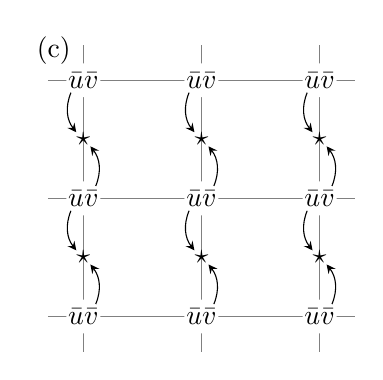
\begin{tikzpicture}[scale=1.5]
        \draw[help lines] (-0.3, -0.3) grid (2.3, 2.3);

        \foreach \x in {0,...,2}
            \foreach \y in {0,...,2}
                \node[circle, inner sep=0pt, fill=white] (uv\x\y) at (\x, \y) {$\bar{u}\bar{v}$};
        \foreach \x in {0,...,2}
            \foreach \y in {0,...,1}
                \node[circle, inner sep=0pt] (duv\x\y) at (\x, \y+0.5) {$\star$};

        \path[stealth-] (duv00.south east) edge[bend left] (uv00.north east);
        \path[stealth-] (duv10.south east) edge[bend left] (uv10.north east);
        \path[stealth-] (duv20.south east) edge[bend left] (uv20.north east);
        %\path[stealth-] (duv30.south east) edge[bend left] (uv30.north east);
        \path[stealth-] (duv01.south east) edge[bend left] (uv01.north east);
        \path[stealth-] (duv11.south east) edge[bend left] (uv11.north east);
        \path[stealth-] (duv21.south east) edge[bend left] (uv21.north east);
        %\path[stealth-] (duv31.south east) edge[bend left] (uv31.north east);
        %\path[stealth-] (duv02.south east) edge[bend left] (uv02.north east);
        %\path[stealth-] (duv12.south east) edge[bend left] (uv12.north east);
        %\path[stealth-] (duv22.south east) edge[bend left] (uv22.north east);
        %\path[stealth-] (duv32.south east) edge[bend left] (uv32.north east);
                                                                           
        \path[stealth-] (duv00.north west) edge[bend left] (uv01.south west);
        \path[stealth-] (duv10.north west) edge[bend left] (uv11.south west);
        \path[stealth-] (duv20.north west) edge[bend left] (uv21.south west);
        %\path[stealth-] (duv30.north west) edge[bend left] (uv31.south west);
        \path[stealth-] (duv01.north west) edge[bend left] (uv02.south west);
        \path[stealth-] (duv11.north west) edge[bend left] (uv12.south west);
        \path[stealth-] (duv21.north west) edge[bend left] (uv22.south west);
        %\path[stealth-] (duv31.north west) edge[bend left] (uv32.south west);
        %\path[stealth-] (duv02.north west) edge[bend left] (uv03.south west);
        %\path[stealth-] (duv12.north west) edge[bend left] (uv13.south west);
        %\path[stealth-] (duv22.north west) edge[bend left] (uv23.south west);
        %\path[stealth-] (duv32.north west) edge[bend left] (uv33.south west);
        \node[black] at (-0.25, 2.25) {(c)};
    \end{tikzpicture}
    \label{fig:adv-y-diff}
    \end{subfigure}%
    \caption{%
        A cross-section illustrating the steps in computing the $D_2[(A_2 u) (A_1 v)]$
        term of the first component of the advection. The horizontal and vertical
        velocity component discretization locations are marked by $u$ and $v$,
        respectively. Arrows emanate from a point contributing to a stencil and point to
        the center of the stencil.
        (a) $A_1$ averages $v$ in the $x$ direction, yielding an approximation $\bar{v}$
        at grid vertices (in 3D, centers of cell edges for which $x$ and $y$ are
        constant).
        (b) $A_2$ averages $u$ in the $y$ direction, yielding an approximation $\bar{u}$
        at the same points as (a). The quantities $A_1 v$ and $A_2 u$ are collocated and
        can be directly multiplied to obtain an approximation of $uv$ at locations marked
        $\bar{u}\bar{v}$.
        (c) $D_2$ approximately differentiates $uv$ in the $y$ direction, yielding the
        desired quantity at each point marked $\star$.
        The approximation of $uv$ is also used to compute $D_1[(A_1 v)(A_2 u)]$ in the
        second component of the advection, wherein application of $D_1$ instead yields
        approximations collocated with locations marked $v$ in (a).
    }
    \label{fig:discretization}
\end{figure}


To discretize the Navier-Stokes equations~\eqref{eq:ins-momentum}--\eqref{eq:ins-incomp},
we use a marker-and-cell (MAC) grid~\cite{Welch:1965jv}: for grid cell center $\x_i$,
scalar-valued function $s(\x)$ is discretized at $\x_i$, and component $\e_a\cdot\vec{v}$
of vector-valued function $\vec{v}(\x)$ at $\x_i - \sfrac12h\e_a$, where $\e_a$ is a
canonical basis vector. Define the centered difference operator
\begin{equation*}
    D_a\phi(\x) = \frac{\phi(\x+\sfrac12 h\e_a) - \phi(\x-\sfrac12 h\e_a)}{h},
\end{equation*}
for which, e.g., $D_1$ approximates differentiation in the $x$ direction. The discrete
divergence, gradient, and Laplacian operators use centered differences, resulting in a
2-point stencil for each discrete first derivative and the standard 7-point discrete
Laplacian. We also define the centered average operator
\begin{equation*}
    A_a\phi(\x) = \frac{\phi(\x+\sfrac12 h\e_a) + \phi(\x-\sfrac12 h\e_a)}2.
\end{equation*}
By averaging $u$ in the $y$ direction and $v$ in the $x$ direction, we obtain collocated
approximations to $u$ and $v$ at the center of a cell edge. Averaging, e.g., $u$ in the
$x$ direction yields an approximation to $u$ at the cell center. We can therefore
discretize the components of the advection term $\div(\u\otimes\u)$ by
\begin{equation}\label{eq:advection}
    \div[h](\u\otimes\u) := %D_b[H^{bl}_rH^{am}_s (A_l u^s(\x,\,t)) (A_m u^r(\x,\,t))].
    \left[\begin{array}{c}
        D_1[(A_1 u) (A_1 u)] + D_2[(A_1 v) (A_2 u)] + D_3[(A_1 w) (A_3 u)] \\
        D_1[(A_2 u) (A_1 v)] + D_2[(A_2 v) (A_2 v)] + D_3[(A_2 w) (A_3 v)] \\
        D_1[(A_3 u) (A_1 w)] + D_2[(A_3 v) (A_2 w)] + D_3[(A_3 w) (A_3 w)]
    \end{array}\right].
\end{equation}
The symbol $\div[h]$ represents the discrete divergence operator.  Figure~%
\ref{fig:discretization} illustrates the steps in computing $D_2[(A_1 v)(A_2 u)]$, which
appears in the first component in~\eqref{eq:advection}. Morinishi \latin{et al}.\ show
that this scheme, $Div. - S2$ in their parlance, is conservative under the assumption
that $\u$ is discretely divergence-free~\cite{Morinishi:1998us}.

To advance the solution, we use either the backward-forward Euler-based scheme~%
\cite{Ascher:1997tm} or the 2-stage scheme described by Peskin~\cite{Peskin:2002go},
modified to advance structures using the newest velocities. The modification makes these
schemes first-order in time, but allow us to separate the Eulerian update from the
Lagrangian update by requiring only information at the beginning of the timestep to
evaluate forces and moving the structure at the end of the timestep. For the
backward-forward Euler scheme, discretizing~\eqref{eq:ins-momentum} to advance time to
$t+\timestep$, yields linear solves of Helmholtz type,
\begin{equation}\label{eq:disc-momentum}
    (I - \timestep\rho^{-1}\mu \laplacian_h) \u^\ast = \u^n - \timestep\left[\div[h]\left(\u^n\otimes\u^n\right) + \rho^{-1}\left(\f^{n+1} - \grad[h]p^n\right)\right] \quad\text{in}~\domain, \\
\end{equation}
with boundary conditions
\begin{equation}\label{eq:disc-bdy}
    \u^\ast = \u^{n+1}_b + \timestep \grad[h] q^{n} \quad\text{on}~\partial\domain,
\end{equation}
where superscripts denote the time step, $\u_b$ is velocity boundary data, $\laplacian_h$
and $\grad[h]$ are the discrete Laplacian and gradient, respectively, and $q$ is
described below. The force density $\f^{n+1}$ is advanced explicitly. The intermediate
velocity field $\u^\ast$ may not be divergence-free. To obtain a velocity field that
satisfies~\eqref{eq:ins-incomp}, we use projection method II (PmII) of Brown, Cortez, and
Minion~\cite{Brown:2001bq}. PmII updates the pressure
\begin{equation*}
    p^{n+1} = p^n + (\rho I - \timestep\mu\laplacian_h)q^{n+1},
\end{equation*}
and generates the divergence-free velocity field
\begin{equation}\label{eq:vel-update}
    \u^{n+1} = \u^\ast - \timestep\grad[h]q^{n+1}
\end{equation}
using pseudo-pressure $q^{n+1}$, which satisfies
\begin{equation}
\begin{alignedat}{2}
    &\alpha k \laplacian_h q^{n+1} = \div[h]\u^\ast &&\quad \text{in}~\domain, \\
    &\n\cdot\grad[h] q^{n+1} = 0                    &&\quad \text{on}~\partial\domain.
\end{alignedat}
\end{equation}
The velocity update~\eqref{eq:vel-update} provides the boundary conditions~%
\eqref{eq:disc-bdy} using a lagged value of the pseudo-pressure. The 2-stage RK method
consists of a backward-forward Euler step followed by a Crank-Nicolson-midpoint step,
which involves only minor modifications to~\eqref{eq:disc-momentum}. In total, we perform
3 Helmholtz solves and 1 Poisson solve per RK stage.

We employ preconditioned conjugate gradients (PCG) to perform the solves. We use
Chebyshev iteration as a preconditioner for the Helmholtz solves and as an error
smoothing procedure and direct solver for multigrid (MG) to precondition the Poisson
solve. Chebyshev iteration is a generalization of weighted Jacobi iteration which
requires only the ability to perform sparse matrix polynomial-vector multiplication.
Chebyshev iteration (MG) PCG is therefore parallelized by using a parallel sparse
matrix-vector multiplication routine with Horner's method to evaluate the polynomials.

In the case of a triply periodic domain, it is clear that the linear solves involve
symmetric matrices. For Dirichlet or Neumann boundaries, we extrapolate using values at
the neighboring grid points and boundary data to fill ghost points. In these situations,
the standard discrete second derivative may actually approximate some non-unit multiple
of its continuous counterpart near the boundary. To account for this but maintain
symmetry of the Helmholtz matrices, we scale equations involving near-boundary values,
excluding the offending discrete second derivative and ghost cell terms. The trade-off is
3 extra diagonal matrix-vector multiplications per RK stage for the ability to use PCG
for the linear solves. For details, see~\ref{sec:boundary-correction}.

% vim: cc=90 tw=89

\section{Force models}\label{sec:force}

In this section, we describe the various forms of force density used in our simulations
and give analytic expressions for each. We consider four kinds of energy densities:
(damped) spring forces, tensions, dissipative forces, and Canham-Helfrich bending forces.
We combine these for the different types of cells used in our simulations.

For simplicity in describing these forces, we adopt the Einstein summation notation in
this section. A Greek letter featuring as a subscript and superscript within a term
indicates summation over ${1,\,2}$ for that letter. For example, we write the vector of
surface coordinates in terms of its components as $\qs = \q[\alpha]\e_\alpha$. We also
adopt the comma notation for partial differentiation, where subscripts following a comma
indicate partial differentiation with respect to the corresponding coordinates, e.g.,
$\phi_{,\alpha\beta} = \partial^2\phi/\partial\q[\alpha]\partial\q[\beta]$.

We begin with Hookean and damped spring forces, which are the simplest of the forces we
consider. The spring force density takes the form
\begin{equation}
    \F_\text{spring} = -k (\X - \X') - \eta(\vec{\dot{X}}-\vec{\dot{X}}').
\end{equation}
where $\X'$ is the tether location, $\vec{\dot{X}}$ is the surface velocity,
$\vec{\dot{X}}'$ is the prescribed velocity, $k$ is the spring constant, and $\eta$ is
the damping constant.  It is common practice to treat each spring as an individual, so
that the quadrature weight $\weight[A]$ is absorbed into the coefficients, and $k$ has
units of force per length and $\eta$ units of force-time per length. Implementation of
these forces requires no geometric information outside of positions and velocities.

Detailed energy models are unavailable for the endothelium, but endothelial cells are
strongly bound to the subendothelium. We take a simple approach by treating the
endothelium as a layer of stiff springs with $k = 2.5\dynpercm$,
$\eta = \scinot{1}{-7}\dynsecpercm$, and zero prescribed velocity. In Section~%
\ref{sec:whole-blood}, we compare different choices for $\X'$.

Next, we consider tension, which generates forces based on stretching or compressing
and relative direction of the surface tangent vectors. We construct the \emph{metric
tensor}, $\metric_{\alpha\beta} = \X_{,\alpha}\cdot\X_{,\beta}$, which encodes local
information about distance and area. Its inverse, denoted by $\metric^{\alpha\beta}$, is
called the dual metric.  Likewise, we construct a metric tensor for the reference
configuration, $\reference\metric_{\alpha\beta}$, and its dual. The invariants of the
Green-Lagrange strain tensor,
\begin{equation}
    \epsilon_\alpha^\beta = \frac12\left(\metric_{\alpha\mu}\reference\metric^{\mu\beta}-\Kronecker_\alpha^\beta\right),
\end{equation}
encode information about relative changes in lengths and areas. Tension energy density
function are often expressed in terms of the invariants $I_1 = 2\epsilon_\mu^\mu$ and
$I_2 = 4\epsilon + I_1$, where $\epsilon_\mu^\mu$ and $\epsilon$ are the trace and
determinant of $\epsilon_\alpha^{\smash\beta}$, respectively. $I_1$ and $I_2$ relate to
changes in lengths and areas, respectively, so that any rigid body motion of the
reference configuration results in $I_1 = I_2 = 0$. The tension energy density function,
$W(I_1,\,I_2)$, is therefore a function only of the tangents, $\X_{,\alpha}$. Of
particular interest are the Skalak Law~\cite{Skalak:1973tp}, which was developed
specifically for RBCs, and neo-Hookean tension,
\begin{align}
    W_\text{Sk} &= \frac{E}{4}\left(I_1^2 + 2I_1 - 2I_2\right) + \frac{G}4 I_2^2, \quad\text{and} \\
    W_\text{nH} &= \frac{E}{2}\left(\frac{I_1+2}{\sqrt{I_2+1}}-2\right) + \frac{G}2 \left(\sqrt{I_2+1}-1\right)^2,
\end{align}
respectively. Here, $E$ is the shear modulus, and $G$ is the bulk modulus. The resulting
tension force density is computed~\cite{Maxian:2018ek} via
\begin{equation}\label{eq:tension-force}
    \F_\text{tension} = \frac{1}{\sqrt{\reference\metric}}\left(\sqrt{\reference\metric}s^{\alpha\beta}\X_{,\beta}\right)_{,\alpha},
\end{equation}
where the second Piola-Kirchhoff stress tensor, $s^{\alpha\beta}$, is given by
\begin{equation}
    s^{\alpha\beta} = 2\frac{\partial W}{\partial I_1} \hat{g}^{\alpha\beta} + 2I_2\frac{\partial W}{\partial I_2} g^{\alpha\beta}.
\end{equation}
Because the tension force density is expressed in relation to the reference
configuration, the force is computed by multiplying by quadrature weights for the
reference configuration, which do not change over the course of a simulation.

For RBCs, deformations generate a force density according to the Skalak Law with moduli
$E_\text{rbc} = \scinot{2.5}{-3}\dynpercm$ and $G_\text{rbc} = \scinot{2.5}{-1}\dynpercm$
and reference configuration given by Omori, \latin{et al.}~\cite{Omori:2012hw},
\begin{equation*}
    \vec{\hat{X}}_\text{rbc}(\qs) = 3.91\um\left(\cos\q[1]\cos\q[2]\e_1 + \sin\q[1]\cos\q[2]\e_2 + z\left(\cos^2\q[2]\right)\sin\q[2]\e_3\right),
\end{equation*}
where $z(r) = 0.105 + r - 0.56r^2$. Platelets do not have a purpose-built constitutive
law, but are stiffer than RBCs. We use the neo-Hookean model with
$E_\text{plt} = \scinot{1}{-1}\dynpercm$, $G_\text{plt} = 1\dynpercm$, and an ellipsoid
reference configuration~\cite{Frojmovic:1982wk},
\begin{equation*}
    \vec{\hat{X}}_\text{plt}(\qs) = 1.5\um\cos\q[1]\cos\q[2]\e_1 + 1.5\um\sin\q[1]\cos\q[2]\e_2 + 0.55\um\sin\q[2]\e_3.
\end{equation*}

These cells also respond to changes in the curvature of the membrane. To compute bending
force density, we first construct the unit normal vector by taking the cross product of
the tangent vectors and normalizing:
\begin{equation}\label{eq:unit-normal}
    \n = \frac{1}{\sqrt{\metric}} (\X_{,1}\times\X_{,2}).
\end{equation}
The tensor $b_{\alpha\beta} = \n\cdot\X_{,\alpha\beta}$ encodes information about the
curvature of the surface. The principle curvatures are the eigenvalues of the
\emph{shape tensor}, $K_\alpha^\beta = b_{\alpha\mu}\metric^{\mu\beta}$, with
$2H = K_\mu^\mu$ the total curvature, and $K$ the Gaussian curvature. The Canham-Helfrich
force density takes the form~\cite{Zhongcan:1989ue}
\begin{equation}\label{eq:bending-force}
    \F_\text{CH} = -4\kappa\left(\laplacian(H-H')+2(H-H')(H^2-K+HH')\right)\n,
\end{equation}
where $\laplacian$ is the Laplace-Beltrami operator. The constants $\kappa$ is the
bending modulus in units of energy, and $H'$ is the spontaneous or preferred curvature.
%$H' = 0$ is a common choice, so that the surface attempts to become more spherical, but
%we also use $H' = \hat{H}$, the reference curvature, so that the surface prefers to be in
%its reference configuration.
We can compute $H$ and $K$ using the formulas above, but
$\laplacian H$ requires up to fourth derivatives of $\X$. In lieu of computing
higher-order derivatives, we compute $H$ and apply the discrete Laplace-Beltrami
operator.

RBCs generate a relatively weak response to changes in curvature. We use a bending
modulus of $\kappa_\text{rbc} = \scinot{2}{-12}\si{erg}$ and a preferred curvature
$H' = 0$ for RBCs. RBCs therefore tend to locally flatten their membranes. For platelets,
we use a larger bending modulus of $\kappa_\text{plt} = \scinot{2}{-11}\si{erq}$ and
a preference for its reference configuration, $H' = \hat{H}$. Together with the
neo-Hookean tension above, this maintains a fairly rigid platelet.

Finally, we consider dissipative forces, which cause the membrane to exhibit a
viscoelastic response to strain. With surface velocity $\vec{\dot{X}}$, the metric tensor
changes in time according to 
\begin{equation}
    \dot{\metric}_{\alpha\beta} = \vec{\dot{X}}_{,\alpha}\cdot\X_{,\beta} + \X_{,\alpha}\cdot\vec{\dot{X}}_{,\beta}.
\end{equation}
The dissipative force density takes the form~\cite{Rangamani:2012hi}
\begin{equation}\label{eq:dissip-force}
    \F_\text{dissip} = \frac{\nu}{\sqrt{\metric}}\left(\sqrt{\metric}\metric^{\alpha\mu}\dot{\metric}_{\mu\lambda}\metric^{\lambda\beta}\X_{,\beta}\right)_{,\alpha},
\end{equation}
where $\nu$ is the membrane viscosity. We imbue only the RBC with viscoelasticity. While
Evans and Hochmuth suggest a viscosity of approximately $\scinot{1}{-3}\dynsecpercm$~%
\cite{Evans:1976tx}, we find this to be prohibitively expensive and instead use
$\nu_\text{rbc} = \scinot{2.5}{-7}\dynsecpercm$.

Rewriting~\eqref{eq:tension-force},~\eqref{eq:dissip-force}, and the Laplace-Beltrami
operator in~\eqref{eq:bending-force} in terms of first and second derivatives with
respect to parametric variables,
\begin{equation}\label{eq:expanded-op}
    \frac1{\sqrt{\metric}}\left(\sqrt{\metric}D^\alpha_\mu \metric^{\mu\beta}\phi_{,\beta}\right)_{,\alpha}
    = \left[\left(D^\alpha_\mu \metric^{\mu\beta}\right)_{,\alpha} + \frac{\metric_{,\alpha}}{2\metric}D^\alpha_\mu \metric^{\mu\beta}\right]\phi_{,\beta}+D^\alpha_\mu \metric^{\mu\beta}\phi_{,\alpha\beta},
\end{equation}
with $D^\alpha_\mu = s^{\alpha\beta}\metric_{\beta\mu}$,
$D^\alpha_\mu = \nu \metric^{\alpha\beta}\dot{g}_{\beta\mu}$, and
$D^\alpha_\mu = \delta^\alpha_\mu$,
respectively, we find that we require only discrete first and second derivative operators
to compute a wide variety of forces. The following section describes our methods for
reconstructing cell surfaces from a set of points and discretizing the necessary
differential operators.


\section{Geometry of reconstructed surfaces}\label{sec:surfaces}

From the previous section, we have analytic expressions for the Lagrangian force density,
$\F$. The RBC and platelet force models require first and second derivatives along their
surfaces. Additionally, The IB force spreading operation requires quadrature weights for
the surfaces. This section finishes where we left off by discussing the construction of
the necessary discrete linear operators and quadrature weights $\weight[A]$ through the
use of RBF-based methods.

\subsection{Surface reconstruction with radial basis functions}\label{sec:rbf-interpolation}

Radial basis functions (RBFs) are a meshfree approach to scattered data approximation
where structural information is encoded purely as point-wise distances. With some
exceptions, they are an appropriate tool for interpolation at arbitrary locations. This
contrasts with, \latin{e.g.}, polynomials, where points must be chosen at grid vertices,
or spherical harmonics, for which special node sets are typically used. RBFs are a viable
approach for representing cells on par with Fourier methods~\cite{Shankar:2013ki}. They
are therefore appealing for representing blood cells.

Because our choice of force model for the endothelium does not require geometric
information, we limit the discussion to RBCs and platelets, which are topologically
spherical. The 2-sphere, $\sphere$, has parametrization
\begin{equation*}
    \Xp(\theta,\,\varphi) =
    \left[\begin{array}{c}
        \cos\theta\cos\varphi \\
        \sin\theta\cos\varphi \\
        \sin\varphi
    \end{array}\right],
\end{equation*}
$(\theta,\,\varphi)\in(-\pi,\,\pi]\times[-\pi/2,\,\pi/2]$.
Let $\data\sites = \{(\data\theta_i,\,\data\varphi_i)\}$ be a set of $\data\cardinality$
distinct \emph{data sites}, defined by the Bauer spiral~\cite{Bauer:2000km},
\begin{equation}\label{eq:bauer-spiral}
    \begin{aligned}
        &\varphi_j = \sin^{-1}(-1 + (2i + 1) / N), \\
        &\theta_j = \modulo\left(\sqrt{N\pi}\varphi_j + \pi,\,2\pi\right) - \pi,
    \end{aligned}
\end{equation}
where $N$ is the number of points, and $\modulo(a,\,b) = a - b\floor{a/b}$ is the modulo
function. Let $\data\Xp_i = \Xp(\theta_i,\,\varphi_i)$ for each
$(\theta_i,\,\varphi_i) \in \data\sites$. Suppose we wish to approximate $\psi(\Xp)$,
defined on $\sphere$. From \emph{basic function} $\phi$, we form our interpolatory basis
with the RBFs $\phi(\|\Xp-\data\Xp_i\|)$, $i=1,\,\ldots,\,\data\cardinality$. Attractive
choices for $\phi$ are the polyharmonic splines (PHS),
\begin{equation*}
    \text{PHS:}\quad\phi(r) = \begin{cases}
        r^{2k} \log r, \\
        r^{2k+1},
    \end{cases}
    \quad\text{for}\ k\in\mathbb{N},
\end{equation*}
which do not require a shape parameter, unlike Gaussian or multiquadric kernels~%
\cite{Fasshauer:2007ui}. However, PHS are finitely differentiable and conditionally
positive definite; they require additional polynomial terms up to degree $k$ to guarantee
a unique interpolant. Heuristically, $\data\cardinality$ is chosen so that data sites
outnumber polynomials at least 2-to-1 to maintain reasonable conditioning. On $\sphere$,
the polynomials are spherical harmonics. We denote the polynomials by $p_k(\Xp)$,
$k=1,\,\ldots,\,\poly\cardinality$. The interpolant takes the form
\begin{equation}\label{eq:rbf-interp}
    s(\Xp)
    = \sum_{i=1}^{\data\cardinality} c_i \phi(\|\Xp-\data\Xp_i\|)
    + \sum_{k=1}^{\poly\cardinality} d_k p_k(\Xp),
\end{equation}
and exactly recovers $\psi$ at each of the data sites,
$s(\data\Xp_j) = \psi(\data\Xp_i)$, for $j = 1,\,\ldots,\,\data\cardinality$. We further
constrain the coefficients $c_i$ so that the polynomials recover polynomial data,
\begin{equation}
    \sum_{i=1}^{\data\cardinality} c_i p_k(\data\Xp_i) = 0.
    \label{eq:constraints}
\end{equation}
Collecting the values $\Phi=(\phi(\|\data\Xp_j-\data\Xp_i\|))$, $P=(p_k(\data\Xp_j))$,
$\arr{c} = (c_i)$, $\arr{d} = (d_k)$, and $\arr{\psi} = (\psi(\data\Xp_j))$, we form
the dense symmetric block system
\begin{equation}\label{eq:rbf-interp-matrix}
    \left[\begin{array}{cc}
            \Phi & P \\ P^T & 0
    \end{array}\right]\left[\begin{array}{c}
            \arr{c} \\ \arr{d}
    \end{array}\right] = \left[\begin{array}{c}
            \arr{\psi} \\ \arr{0}
    \end{array}\right],
\end{equation}
where the matrix block $0$ is the $\poly\cardinality\times\poly\cardinality$ zero matrix
and $\arr{0}$ is a vector of $\poly\cardinality$ zeros. Because $\data\sites$ is fixed,
we need only construct this matrix and compute its factors once.

For RBC and platelet parametrizations, we identify the point $\X(\theta,\,\varphi,\,t)$
on $\interface$ with the point $\Xp(\theta,\,\varphi)$ on $\sphere$. Each component of
$\X$ is a function defined on $\sphere$. By sampling $\X$ at each point in $\data\sites$,
we can approximately reconstruct the surface by interpolating each of the components. It
is clear from Equations~\eqref{eq:skalak-law}--\eqref{eq:dissip-energy} that computing
the force densities requires values of $I_1$, $I_2$, and $H$, among others. These values
are derived from the first and second derivatives of $\X$. See~\ref{sec:forces} for
details. To meet the smoothness requirements for evaluating the force densities, we use
$\phi(r) = r^7$ for RBCs and platelets, with up to $5\th$ order spherical harmonics for
RBCs and just the constant polynomial for platelets. While this does not guarantee a
unique interpolant for the platelet, the resulting system~\eqref{eq:rbf-interp-matrix} is
invertible nonetheless. The interpolants are then thrice differentiable. We next describe
the construction of the necessary discrete differential operators.

\subsection{Discrete linear surface operators}

Let $\L$ be a linear operator. In particular, we are interested in the first- and
second-order partial differential operators, $\partial/\partial\theta$,
$\partial^2/\partial\theta\partial\varphi$, \latin{etc}. We approximate $\L\psi$ by
applying $\L$ analytically to the interpolant $s$ defined in Equation~%
\eqref{eq:rbf-interp}. This is straightforward, given a parametrized metric. For
$\sphere$, this is
\begin{equation}\label{eq:sphere-metric}
    \begin{aligned}
    \|\Xp(\theta_j,\,\varphi_j) - \Xp(\theta_i,\,\varphi_i)\|
    &= \sqrt{2(1 - \cos\varphi_j\cos\varphi_i\cos(\theta_j-\theta_i) - \sin\varphi_j\sin\varphi_i)} \\
    &= \sqrt{2(1-\Xp(\theta_j,\,\varphi_j)\cdot\Xp(\theta_i,\,\varphi_i))}.
\end{aligned}
\end{equation}
However, evaluating $\L s$ at each data site involves dense operations against a
$\data\cardinality\times(\data\cardinality+\poly\cardinality)$ matrix. Depending on the
needs of the simulation, the number of data sites may be large.  In the interest of
saving memory and time for such cases, we opt instead to use fewer data sites to
reconstruct the surface, and choose a larger set of $\sample\cardinality$ \emph{sample
sites}, $\sample\sites$, at which to evaluate $\L$. We must then also consider $\L$ the
identity operator in order to obtain $\X$ at sample sites. Evaluating $\L s$ at each
sample site and collecting values $\L\Phi = (\L\phi(\|\Xp-\data\Xp_i\|)|_{\Xp=\Xpsj})$
and $\L P = (\L p_k(\Xp)|_{\Xp=\Xpsj})$, where $\Xpsj = \Xp(\theta_j,\,\varphi_j)$ for
each $(\theta_j,\,\varphi_j)\in\sample\sites$,\comment{}{$\Xpsj$ is \emph{not} a sample
site, but $(\theta_j,\,\varphi_j)\in\sample\sites$ is.} we have
\begin{equation}\label{eq:rbf-operator}
    \begin{aligned}
    \left[\begin{array}{cc}
            \L\Phi & \L P
    \end{array}\right]\left[\begin{array}{c}
            \arr{c} \\ \arr{d}
    \end{array}\right] &\hphantom{:}=
    \left[\begin{array}{cc}
            \L\Phi & \L P
    \end{array}\right]\left[\begin{array}{cc}
            \Phi & P \\ P^T & 0
    \end{array}\right]^{-1}\left[\begin{array}{c}
            \arr{\psi} \\ \arr{0}
    \end{array}\right] \\ &:=
    \left[\begin{array}{cc}
            L & \ast
    \end{array}\right]\left[\begin{array}{c}
            \arr{\psi} \\ \arr{0}
    \end{array}\right],
\end{aligned}
\end{equation}
where we have used Equation~\eqref{eq:rbf-interp-matrix} to substitute for $\arr{c}$ and
$\arr{d}$. The matrix $L$ is the discrete analogue of $\L$ applied at each sample site.
It is important to note that $L$ is completely independent of the function $\psi$; in
fact, it depends only on the functions $\phi$ and $p_k$, the fixed data sites
$\data\sites$, and the fixed sample sites $\sample\sites$.  The block marked by $\ast$ is
multiplied by zeros, and can be discarded. We compute a separate $L$ for each operator
$\L$ as a preprocessing step, and simply apply these matrices to any function that needs
to be evaluated or differentiated. It is also straightforward to generate versions of $L$
that produce derivatives at the data sites simply by replacing $\Xpsj$ with $\data\Xp_j$
in the above discussion. With these operators in hand, the force densities are readily
discretized. The quantities $I_1$, $I_2$, and $H$ in Section~\ref{sec:energy} are
calculated using local first and second derivatives. Application of the dense discrete
differential operators is performed in parallel with a parallel implementation of
\texttt{BLAS}. Lagrangian forces can therefore be computed in parallel with few thread
synchronizations.

We now have a method for computing a suitable set of points and for discretizing $\F$ for
use in~\eqref{eq:ib-spread}. To compute a force from a force density, we need to
approximate quadrature weights, or surface patch areas, for each sample site. The
following section is devoted to computing quadrature weights $\weight[j]$ for each
sample site using RBFs.

% vim: cc=90 tw=89

\subsection{Surface area weights via RBF quadrature}\label{sec:rbf-quadrature}

We also use the known parametrization of $\sphere$ to compute RBF-based quadrature weights
on $\sphere$ as a preliminary step in computing quadrature weights on any surface
diffeomorphic to $\sphere$, namely, RBC and platelet membranes.

As before, consider a function $\psi(\Xp):\sphere \to \mathbb{R}$, and $\phi: \sphere \times \sphere \to \mathbb{R}$ be a radial kernel defined on the sphere. We wish to find a set
of quadrature weights $\omega_j$ such that
\begin{equation}\label{eq:quad-desire}
    \int_{\sphere} \psi(\Xp) \d\Xp \approx \sum_{j=1}^{\sample\cardinality} \omega_j \psi(\Xpsj).
\end{equation}
We use a variant of the technique described by Fuselier \latin{et al.}~%
\cite{Fuselier:2013coba}.  Choosing $\psi(\Xp) = \phi(\|\Xp-\sample\Xp_i\|)$ for each
$\sample\Xp_i$, Equation~\eqref{eq:quad-desire} becomes
\begin{equation}
    \sum_{j=1}^{\sample\cardinality} \omega_j \phi(\|\Xpsj-\sample\Xp_i\|)
    \approx \int_{\sphere}\phi(\|\Xp-\sample\Xp_i\|) \d\Xp := \L\phi|_{\Xp=\sample\Xp_i}.
    \label{eq:cond1t}
\end{equation}
However, because the spherical metric~\eqref{eq:sphere-metric} depends only on the angle
between two points, $\L\phi$ is constant over
the sphere. We therefore expect the right-hand side to be a constant, which we denote
$-I_\phi$. We require further that $\omega_j$ sum to the surface area of $\sphere$,
\latin{i.e.},
\begin{equation}
    \sum_{j=1}^{\sample\cardinality} \omega_j  = 4\pi.
    \label{eq:weight-sum}
\end{equation}
Treating $I_\phi$ as an unknown scalar, we rewrite the constraints~\eqref{eq:cond1t} and%
~\eqref{eq:weight-sum} as a symmetric block linear system for $\omega_j$. Let
$\Phi = (\phi(\|\Xpsj - \sample\Xp_i\|))$, $\arr{\omega} = (\omega_j)$, $\arr{0}$ 
be a vector of $\sample\cardinality$ zeros, and $\arr{1}$ be defined similarly with ones.
Then
\begin{equation}\label{eq:rbf-quadrature}
    \left[\begin{array}{cc}
            \Phi & \arr{1} \\ \arr{1}^T & 0
    \end{array}\right]\left[\begin{array}{cc}
            \arr{\omega} \\ I_\phi
    \end{array}\right] = \left[\begin{array}{c}
            \arr{0} \\ 4\pi
    \end{array}\right].
\end{equation}
$I_{\phi}$ serves as a Lagrange multiplier that enforces~\eqref{eq:weight-sum}, and
$-I_\phi$ is a good approximation to $\L\phi$. By choosing $\phi(r) = r$, we guarantee a
unique solution and obtain weights that we observe to converge at 3\textsuperscript{rd}
order. It is possible to improve the order of the quadrature weights by increasing the
order of the PHS RBF at the potential cost of poorer conditioning and either loss of
invertibility or requiring knowledge of higher-order moments~\cite{Fuselier:2013coba}.

Having described the computation of quadrature weights for $\sphere$, we now
describe how to compute quadrature weights for $\interface$, which has parametrization
$\X(\theta,\,\varphi)$ and Jacobian $J(\theta,\,\varphi)$. The point
$\X(\theta,\,\varphi)$ on the cell and $\Xp(\theta,\,\varphi)$ share surface coordinates
and the determinant of the Jacobian for the spherical coordinate mapping (for radius 1) is simply $\cos\varphi$.  We use a change of variables to
express the infinitesimal area $\d\X$ as
\begin{equation}\label{eq:quad-cov}
    \d\X
    = J(\theta,\,\varphi)\d\qs
    = J(\theta,\,\varphi)\sec\varphi\d\Xp,
\end{equation}
where $\d\qs$ is an infinitesimal area in parameter space. The weights $\omega_j$ found
above are discrete analogues of $\d\Xp$ at $\sample\Xp_j$. The discrete analogue of
$\d\qs$ at the $j^\text{th}$ sample site,
\begin{equation*}
    \sigma_j=\sec\varphi_j\omega_j,
\end{equation*}
can be computed at the outset of a simulation. To avoid numerical issues, we require that
$\cos\varphi_j \neq 0$ for each sample site. This is true everywhere on $\sphere$ except
the poles, $(0,\,0,\,\pm1)$. The Bauer spiral~\eqref{eq:bauer-spiral} conveniently avoids
these points. We now arrive our weights for $\interface$. At $\X_j$, we have
\begin{equation}
    \weight[j] = \sigma_j J_j,
\end{equation}
where $J_j = J(\theta_j,\,\varphi_j)$. Computing $\weight[j]$ given $\sigma_j$ and $J_j$
amounts to a single multiplication, which can be done trivially in parallel.

%The methods described in this section are not restricted to the sphere. In Section~%
%\ref{sec:whole-blood}, we simulate the endothelium, which is a topological torus, due to
%the periodicity of the domain. Though we do not need geometric information for the force
%model used for the endothelium, the RBF methods above are also applicable to the torus,
%and therefore the endothelium. The following section describes the necessary
%modifications for the endothelium. We use a local variation of these methods as part of
%the simulation initialization process, described in Section~\ref{sec:blood-init}.


\subsection{A note on the endothelium}
While our choice of force density for the endothelium does not require surface
reconstruction or quadrature weights, the methods described above are equally applicable.
The periodicity of $\domain$ makes the endothelium a topological torus. The 4-dimensional
torus, $\mathbb{T}$, with parametrization
\begin{equation*}
    \Xp(\qs) = \cos\q[1]\e_1 + \sin\q[1]\e_2 + \cos\q[2]\e_3 + \cos\q[2]\e_4,
\end{equation*}
for $\qs\in\sites=[0,\,2\pi)^2$, is orientation agnostic and homogeneous. It has surface
area $4\pi^2$ and Jacobian $\tilde{J} = 1$. It is, however, trivial to choose a set of
points on $\mathbb{T}$ that generate equal quadrature weights without the need to solve a
system like~\eqref{eq:quadrature-weights}--\eqref{eq:quadrature-constraint}. Any regular
grid suffices, but we generate a set of $N$ points, whether used for interpolation or
not, with the spiral
\begin{align*}
    \q^2_i &= 2\pi (i-1)/N, \\
    \q^1_i &= \modulo\left(\left\lceil\!\sqrt{N}\mskip\thinmuskip\right\rceil\theta^2_i,\,2\pi\right).
\end{align*}
Using distances between points
on $\mathbb{T}$ to construct RBFs allow for the interpolation of, and quadrature on, any
toroidal surface. However, care needs to be taken in applying the constructed discrete
operators to a ``flat'' torus, such as the endothelium. If, for example, $L$ is the
discrete analogue of $\L$ evaluated at sample site $\sample\qs$ and the interpolated
function $\psi(\qs)$ decomposes into
\begin{equation*}
    \psi(\qs) = \bar{\psi}(\qs) + \text{periodic part},
\end{equation*}
where $\bar{\psi}$ is known, aperiodic, and independent of time, then
\begin{equation*}
    \L\psi(\sample\qs)
    \approx \L\bar{\psi}(\sample\qs) + L\left(\data{\vec{\psi}} - \data{\vec{\bar{\psi}}}\right)
    := L\data{\vec{\psi}} + \epsilon,
\end{equation*}
where $\data{\vec{\psi}}$ and $\data{\vec{\bar{\psi}}}$ are vectors formed by evaluating
$\psi$ and $\bar{\psi}$, respectively, at each point in $\data\sites$. Computing
$\epsilon$ for each sample site can be done simultaneously, resulting in the vector
$\vec{\epsilon}$. A correction like $\vec{\epsilon}$ may be needed for each linear
operator.
